\documentclass[a4paper, 12pt]{article}
\usepackage[T1]{fontenc}
\usepackage{lmodern}
\usepackage{color}
\usepackage{amsfonts}
\usepackage{epstopdf}
\usepackage{matlab}
\usepackage{booktabs}
%\documentclass{book}
\usepackage{blindtext}
\usepackage{hyperref}
\usepackage[brazil]{babel}
\usepackage{amssymb}
\usepackage[utf8]{inputenc}
\usepackage{amsmath}
\usepackage{indentfirst}
\usepackage{graphicx}
\usepackage{listings}
\usepackage{tcolorbox}
\usepackage{upgreek}
\usepackage{multicol,lipsum}
\usepackage[a4paper,
top=3cm, left=3cm, bottom=3cm, right=3cm]{geometry}
\usepackage{setspace}
\usepackage{multirow}
\usepackage{float}
\usepackage[dvipsnames]{xcolor}
\usepackage[table]{xcolor}
%\usepackage{pdflscape}
\usepackage[DIV=15]{typearea}
\usepackage[nottoc]{tocbibind}
\usepackage[sort,numbers]{natbib}
%\usepackage{cite}
\usepackage{matlab}

\usepackage[utf8]{inputenc}
\usepackage[T1]{fontenc}
\usepackage{lmodern}
\usepackage{graphicx}
\usepackage{color}
\usepackage{hyperref}
\usepackage{amsmath}
\usepackage{amsfonts}
\usepackage{epstopdf}
\usepackage[table]{xcolor}
\usepackage{matlab}

\lstdefinestyle{python}{
  language=Python,
  basicstyle=\ttfamily,
  keywordstyle=\color{blue},
  stringstyle=\color{magenta},
  commentstyle=\color{gray},
  numbers=left,
  numberstyle=\tiny\color{gray},
  stepnumber=1,
  numbersep=5pt,
  backgroundcolor=\color{white},
  showspaces=false,
  showstringspaces=false,
  showtabs=false,
  frame=single,
  rulecolor=\color{black},
  tabsize=4,
  captionpos=b,
  breaklines=true,
  breakatwhitespace=false,
  title=\lstname,
  escapeinside={\%*}{*)},
  morekeywords={self},
  emph={MyClass,__init__},
  emphstyle=\color{red}
}


\documentclass[letterpaper]{article}
% bib pack %%%%%%%%%%%%%%%%%%%%%%%%%%%%%%%%%%%%%%%%%%%%%%%%%%%%%%%%%%%%%%%%%%%%%
\usepackage[utf8]{inputenc}
\usepackage{geometry}
    \geometry{left=3cm,right=2cm,top=2cm,bottom=2cm}
%
\usepackage[spanish]{babel}
%
\usepackage[fixlanguage]{babelbib}
    \bibliographystyle{babunsrt}
%
\usepackage{url}

\begin{document}
%\maketitle

\begin{titlepage}
	\begin{center}
		

\vspace{10pt}
%\begin{figure}[H][!ht]
%\centering
%
\includegraphics{puc-rio-logo.png}

%\end{figure}
\begin{figure}[!ht]
\centering

\includegraphics{images/puc-rio-logo.png}
\end{figure}
\huge{Análise de Séries Temporais}
        \vspace{70pt}
        
		\textbf{ENG1469}
		\textbf{\large{\\ }}
		
		\vspace{30pt}
		\textbf{\small{\\Lista Prática 01}}
		\vspace{75pt}
		
	\end{center}
	
	\begin{flushleft}
		\begin{tabbing}
		Aluno(a)\qquad\qquad\=\>Paloma Fernanda Loureiro Sette - 1621595\\
			Professor(a)\>Cristiano Fernandes\\
	\end{tabbing}
		  
	\end{flushleft}
	\begin{center}
		%\vspace{\fill}
		\vspace{215pt}
		Rio de Janeiro, 03 de Setembro de 2024
	\end{center}
\end{titlepage}
%%%%%%%%%%%%%%%%%%%%%%%%%%%%%%%%%%%%%%%%%%%%%%%%%%%%%%%%%%%
\newpage
\tableofcontents
\thispagestyle{empty}

\newpage
\pagenumbering{arabic}

\newpage

%\newcommand{\listequationsname}{Lista de Equações}
%\newlistof{myequations}{equ}{\listequationsname}
%\newcommand{\myequations}[1]{%
%\addcontentsline{equ}{myequations}{\protect\numberline{\theequation}#1}\par}

%\listofmyequations
\newpage


\newpage

\listoffigures
\thispagestyle{empty}

\newpage
%%%%%%%%%%%%%%%%%%%%%%%%%%%%%%%%%%%%%%%%%%%%%%%%%%%%%%%%%
%%%%%%%%%%%%%%%%%%%%%%%%%%%%%%%%%%%%%%%%%%%%%%%%%%%

\newpage

\thispagestyle{empty}

\newpage

\section*{Introdução}
Este relatório refere-se à primeira lista prática da disciplina de Análise de Séries Temporais (ENG1469) de 2024.2.\\

Para este trabalho, utilizaremos a série temporal relacionada a vendas nominais no varejo de livros, jornais, revistas e papelaria. É possível encontrar esta série no \href{http://ipeadata.gov.br/Default.aspx}{Ipeadata}. (macroeconômico >> Periodicidade >> Mensal >> Consumo e Vendas >> Vendas nominais no varejo de livros, jornais, revistas e papelaria).\\


Para vendas nominais, considera-se a receita bruta de revenda, total e por Unidade da Federação, definida no âmbito da empresa como a receita bruta mensal proveniente da revenda de mercadorias, não deduzidos os impostos incidentes e nem as vendas canceladas, abatimentos e impostos incondicionais. Para varejo considera-se as atividades de revenda, venda sem transformação significativa, de bens de consumo novos e usados, preponderantemente para o consumidor final. O comércio varejista é organizado para vender mercadorias em pequenas quantidades ao consumidor final, representando, portanto, o último elo da cadeia de distribuição. A classificação das atividades do comércio varejista baseia-se na gama de produtos vendidos, sem distinção da forma de comercialização em loja ou fora de loja. Para livros, jornais, revistas e papelaria considera-se o comércio varejista de livros, inclusive didáticos, o comércio varejista de revistas, jornais, revistas e outros impressos, o comércio varejista de artigos de escritório, as bancas de jornais e revistas, o comércio varejista de artigos de papelaria, tais como cadernos, borrachas, lápis, canetas, cartolinas e similares. Não fazendo parte desta classificação o comercio varejista de livros usados, o comércio varejista de selos, o comércio varejista de suprimentos de informática. A base foi fixada como a média das observações no ano de 2022. Nota: A Pesquisa Mensal de Comércio foi iniciada em janeiro de 1995, com o intuito de produzir indicadores que possam acompanhar o desempenho conjuntural do comércio varejista no país, investigando a receita bruta de revenda nas empresas formalmente constituídas de 20 ou mais pessoas ocupadas.\\

\newpage
\subsection{Carregando os dados}
A princípio, é necessário carregar os dados e fazer os devidos tratamentos:

\begin{lstlisting}[style=python]
import pandas as pd

file_path = 'dados.xls' 

data = pd.read_excel(file_path)

data['Data'] = data['Data'].astype(str)

data['Data'] = pd.to_datetime(data['Data'], format='%Y.%m')

data.set_index('Data', inplace=True)

# Dividindo a serie em treino e teste
train = data.iloc[:-12]  # Todas as observacoes exceto as 12 ultimas
test = data.iloc[-12:]   # As ultimas 12 observacoes

\end{lstlisting} \\

No código acima, carregamos os dados do documento XLS original, que contém as colunas Data e Vendas, e dividimos a série em dados de treino e teste. 

\begin{figure}[H]
\centering
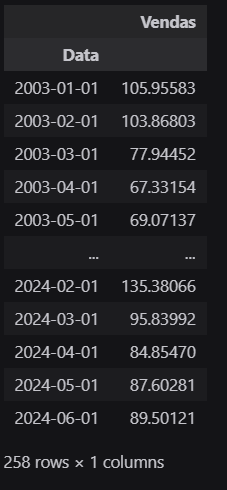
\includegraphics[scale = 0.80]{images/0.1.png}
\label{filtro1}
\caption{Dataframe base - ST}
\end{figure}

A série temporal fornecida pelo IPEA Data referente às vendas nominais no varejo de livros, jornais, revistas e papelaria é expressa como um índice (média de 2022 = 100).\\

Diferentemente de valores absolutos que poderiam ser expressos em milhões, os dados utilizados neste trabalho são índices que indicam o desempenho das vendas em relação a uma média-base estabelecida em 2022. Cada valor na série temporal reflete a proporção ou percentual em relação a essa média-base, com o ano de 2022 estabelecendo o nível de 100.\\

Ao carregar e manipular os dados no Python, os valores mantiveram essa estrutura de índice, o que foi confirmado ao comparar os dados carregados com os exibidos diretamente no site do IPEA Data.\\




%%%%%%%%%%%%%%%%%%%%%%%%%%%%%%%%%%%%%%%%%%%%%%%%%
\section{- Questão 01}
\textbf{Especifique, com todos os detalhes, uma situação prática em que as previsões
da sua série temporal seriam úteis em um processo de tomada de decisão (governamental, empresarial etc).} \\


Podemos explorar uma situação prática onde a previsão da série temporal, que trata das vendas nominais no varejo de livros, jornais, revistas e papelaria, poderia ser útil em um processo de tomada de decisão empresarial. Por exemplo:\\


\textbf{Planejamento de Estoque e Estratégia de Marketing para uma Rede de Livrarias}\\

\begin{itemize}
    \item \textbf{Contexto}\\
    Uma grande rede de livrarias, com filiais em várias cidades do Brasil, está enfrentando desafios na gestão de estoques e na elaboração de campanhas de marketing sazonais. A rede observa que há uma forte sazonalidade nas vendas de livros, jornais, revistas e artigos de papelaria, com picos de vendas em meses específicos, como durante o período de volta às aulas e no final do ano. No entanto, a empresa não consegue prever com precisão essas variações, o que resulta em dois problemas principais:
    \begin{itemize}
        \item \textbf{Excesso de Estoque:} Durante os períodos de baixa demanda, a empresa acaba com um estoque excessivo de produtos, aumentando os custos de armazenamento e riscos de obsolescência.
        \item \textbf{Falta de Estoque: } Durante os picos de demanda, a falta de estoque resulta em perda de vendas e insatisfação dos clientes.
    \end{itemize}
\end{itemize}

\begin{itemize}
    \item \textbf{Objetivo}\\
    Utilizar a previsão da série temporal das vendas nominais para melhorar o planejamento de estoque e otimizar as campanhas de marketing, garantindo que a oferta de produtos esteja alinhada com a demanda prevista.
\end{itemize}

\begin{itemize}
    \item \textbf{Abordagem}
    \begin{enumerate}
        \item \textbf{Previsão das Vendas:} 
        \begin{itemize}
            \item Usando métodos de previsão de séries temporais, como ETS e EWMA, a empresa pode prever as vendas dos próximos meses com base nas tendências históricas e padrões sazonais observados na série temporal.
            \item A previsão ajudará a determinar quantos produtos devem ser estocados em cada filial para evitar excesso ou falta de estoque.
        \end{itemize}
        \item \textbf{Estratégia de Marketing:}
        \begin{itemize}
            \item Com base nas previsões de vendas, a empresa pode planejar campanhas de marketing direcionadas para os períodos de baixa demanda, como promoções ou eventos para atrair clientes durante esses meses.
            \item Durante os períodos de alta demanda, a empresa pode focar em campanhas que incentivem a compra antecipada ou ofereçam pacotes promocionais, maximizando as vendas durante esses picos.
        \end{itemize}
        \item \textbf{Gestão de Estoques:}
        \begin{itemize}
            \item A previsão permitirá à equipe de operações ajustar os pedidos aos fornecedores, garantindo que os produtos cheguem às lojas no momento certo e nas quantidades adequadas.
            \item Isso reduzirá custos de armazenamento e o risco de produtos encalhados ou fora de estoque.
        \end{itemize}
    \end{enumerate}
\end{itemize}
\begin{itemize}
    \item \textbf{Benefícios}
    \begin{itemize}
        \item \textbf{Redução de Custos:}  A empresa poderá reduzir os custos associados ao excesso de estoque e melhorar a eficiência logística.
        \item \textbf{Aumento de Vendas:} Com o estoque adequado e campanhas de marketing bem direcionadas, a empresa pode aumentar as vendas e melhorar a satisfação do cliente.
        \item \textbf{Tomada de Decisão Informada:} A previsão baseada em dados permite que a gerência tome decisões mais informadas e estratégicas, antecipando-se às flutuações de mercado.
    \end{itemize}
\end{itemize}

Neste cenário, a previsão da série temporal das vendas nominais no varejo de livros, jornais, revistas e papelaria é essencial para o planejamento estratégico e operacional da rede de livrarias. A capacidade de prever a demanda futura permite à empresa ajustar suas operações de maneira proativa, resultando em maior eficiência e melhor desempenho financeiro. Esse é um exemplo prático de como a previsão da série pode ser utilizada para influenciar decisões empresariais críticas. 


%%%%%%%%%%%%%%%%%%%%%%%%%%%%%%%%%%%%%%%%%%%%%%%%%
\newpage
\section{- Questão 02}

\textbf{
Obtenha, considerando o período de treinamento da sua ST: \\\\
2.1) O gráfico da série no tempo, observando, por inspeção visual, se há evidências
de tendência, sazonalidade e observações aberrantes (aquelas que destoam
da maioria das observações da S). Tente justificar o porquê da presença das
componentes detectadas visualmente. \\\\
2.2) Gráfico do box-plot de cada um dos meses (todos no mesmo gráfico), para a
para a 1ª diferença da série, interpretando-o.
} \\\\


\subsection{ (i) Gráfico da Série no Tempo}
Primeiro, plotando o gráfico da série temporal no tempo para observar tendências, sazonalidades e possíveis observações aberrantes (outliers), utilizando a biblioteca matplotlib do Python.\\

\begin{lstlisting}[style=python]
# QUESTAO 2
# I)
# Gerando o grafico da serie temporal de treinamento
import matplotlib.pyplot as plt

plt.figure(figsize=(12, 6))
plt.plot(train.index, train['Vendas'], label='Vendas')
plt.title('Serie Temporal de Vendas no Varejo (Periodo de Treinamento)')
plt.xlabel('Ano')
plt.ylabel('Vendas')
plt.legend()
plt.grid(True)
plt.show()
    \end{lstlisting} \\

\begin{figure}[H]
\centering
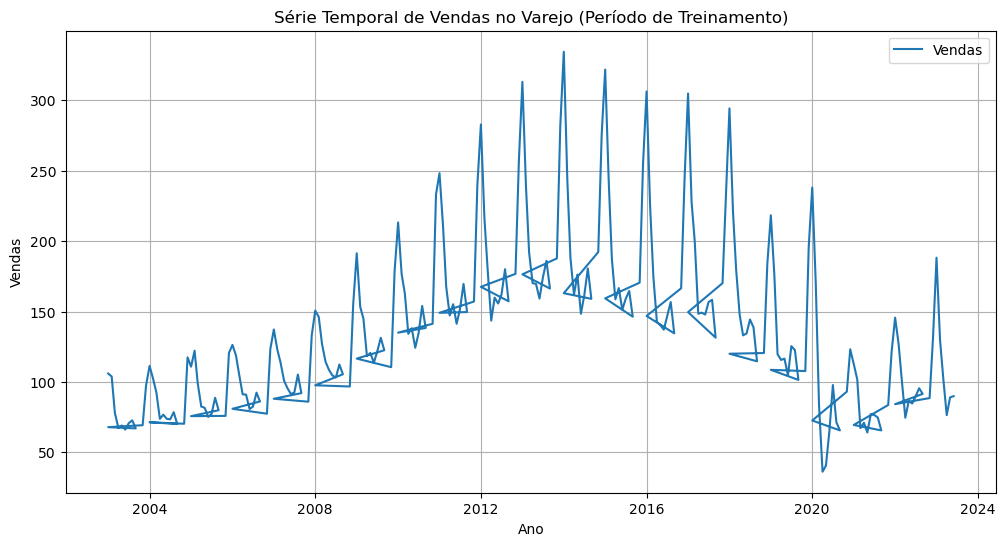
\includegraphics[scale = 0.5]{images/2.1_GraficoST.png}
\label{filtro1}
\caption{Gráfico plotado da ST - Questão 02}
\end{figure}

\textbf{1. Tendência:}\\

No gráfico, é possível observar uma tendência de crescimento geral nas vendas até aproximadamente 2014. A partir desse ponto, parece haver uma estabilização ou até mesmo uma leve queda nas vendas, com uma recuperação gradual após 2021. Esse comportamento pode indicar uma fase de crescimento do mercado, seguida de um período de estabilização e possíveis flutuações.\\

O crescimento nas vendas até 2014 pode ser justificado por uma expansão do mercado de consumo, com mais pessoas comprando livros, jornais, revistas e artigos de papelaria. A estabilização ou leve queda posterior pode refletir uma saturação do mercado ou mudanças nas preferências dos consumidores (por exemplo, migração para meios digitais).\\\\

\textbf{2. Sazonalidade:}\\

O gráfico mostra uma clara sazonalidade, com picos e vales que se repetem anualmente. Esses picos correspondem provavelmente a períodos de alta demanda, como o final do ano (devido às compras de fim de ano) e o início do ano (período de volta às aulas). A regularidade desses picos ao longo dos anos sugere uma forte sazonalidade no comportamento das vendas.\\

Para analisarmos com mais precisão a parte da sazonalidade, podemos observar o gráfico na configuração gerada pelo Ipeadata, com melhor visualização, uma vez que, devido ao grande númoero de dados, o Python não nos proporcionou uma visualização tão clara a respeito da sazonalidade.\\

O gráfico a seguir mostra uma clara sazonalidade, com picos e vales que se repetem anualmente. Esses picos correspondem provavelmente a períodos de alta demanda, como o final do ano (devido às compras de fim de ano) e o início do ano (período de volta às aulas). A regularidade desses picos ao longo dos anos sugere uma forte sazonalidade no comportamento das vendas. A sazonalidade é esperada nesse tipo de mercado, com vendas mais altas em períodos como volta às aulas e fim de ano. Esses padrões sazonais são típicos em mercados voltados para consumidores finais, especialmente em segmentos como papelaria.


\begin{figure}[H]
\centering
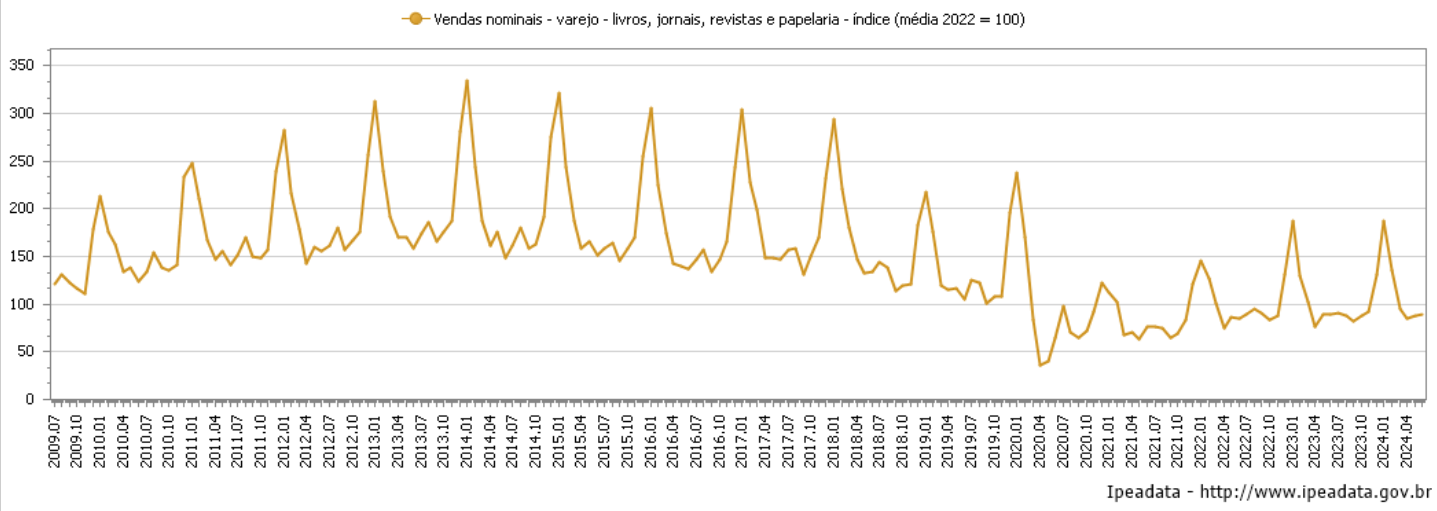
\includegraphics[scale = 0.5]{images/2.1_graficoIpeadata.png}
\label{filtro1}
\caption{Gráfico do Ipeatada}
\end{figure}

Há um pico considerável nas vendas nos meses de janeiro ao longo de todo o período. Esse aumento significativo nas vendas em janeiro pode ser atribuído ao período de volta às aulas. Janeiro é tradicionalmente um mês em que muitas famílias compram materiais escolares, livros didáticos, e outros artigos de papelaria para o novo ano letivo. Isso resulta em um aumento notável nas vendas para lojas de livros, jornais, revistas e papelaria.\\

Além dos picos em janeiro, há um padrão de picos menores, mas ainda significativos, que ocorrem geralmente em julho ou agosto. Esses picos menores podem estar relacionados ao segundo semestre letivo, quando algumas escolas e universidades retomam as aulas após as férias de meio de ano. Durante esse período, os consumidores podem precisar repor ou adquirir novos materiais escolares, livros, e outros itens relacionados à educação. Além disso, julho/agosto também pode coincidir com períodos de lançamento de novas publicações ou promoções de meio de ano nas livrarias, incentivando as vendas.\\\\

\textbf{3. Observações Aberrantes (Outliers):}\\

Há um pico muito elevado nas vendas por volta de 2012/2013, bem acima dos outros picos regulares que ocorrem em janeiro. Esse pico pode ser considerado um outlier, indicando um evento excepcional que impulsionou as vendas nesse período. Isso poderia estar relacionado a uma grande promoção, uma política governamental que incentivou a compra de livros, ou outro evento significativo.\\

Outro possível outlier está em 2020, onde há uma queda abrupta nas vendas seguida por um aumento rápido. A queda drástica durante os primeiros meses de 2020 é particularmente notável. A queda pode ser atribuída à pandemia de COVID-19, que afetou muitas indústrias globalmente. A interrupção das atividades escolares, o fechamento de lojas físicas, e as medidas de quarentena podem ter contribuído para esse comportamento incomum nas vendas. \\

Há também um pico de recuperação em 2021, possivelmente refletindo a retomada das atividades econômicas e educacionais após as restrições da pandemia. Embora não seja tão acentuado quanto o pico de 2012/2013, esse aumento rápido após um período de queda pode ser visto como uma reação aos eventos de 2020, novamente mostrando um comportamento incomum.

 





\subsection{(ii) Gráfico do box-plot}

Agora, precisamos calcular a primeira diferença da série (diferença entre valores consecutivos) e criar um gráfico de box-plot para cada mês:\\


\begin{lstlisting}[style=python]
## 2.2)
# Calculando a primeira diferenca da serie temporal de treinamento
train_diff = train['Vendas'].diff().dropna()

# Adicionando uma coluna para identificar o mes
train_diff = train_diff.to_frame(name='Vendas_Diff')
train_diff['Mes'] = train_diff.index.month

# Gerando o box-plot das diferenças por mes
plt.figure(figsize=(12, 8))
train_diff.boxplot(column='Vendas_Diff', by='Mes', grid=False)
plt.title('Box-Plot das Primeiras Diferencas por Mes')
plt.suptitle('')
plt.xlabel('Mes')
plt.ylabel('Diferencca de Vendas')
plt.show()
    \end{lstlisting} \\

\begin{figure}[H]
\centering
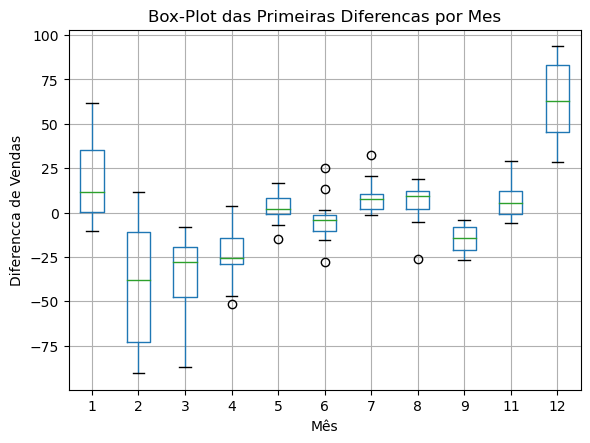
\includegraphics[scale = 0.9]{images/2.2_box-plot.png}
\label{filtro1}
\caption{Gráfico Box-Plot - Questão 02}
\end{figure}

No contexto deste projeto, o gráfico do box-plot das primeiras diferenças por mês nos ajuda a entender como as mudanças nas vendas ocorrem de um mês para o outro ao longo dos anos. Ele permite visualizar a variabilidade e detectar outliers em como as vendas mudam mês a mês, fornecendo insights sobre a estabilidade ou instabilidade do comportamento das vendas em diferentes épocas do ano. O gráfico do box-plot das primeiras diferenças por mês está agregando os dados por mês ao longo de todos os anos.\\


Interpretação do Box-Plot:\\

\textbf{Mês 1 (Janeiro)}:  A mediana é positiva, indicando que, em média, há um aumento significativo nas vendas de dezembro para janeiro. Isso é consistente com o aumento das vendas devido à temporada de volta às aulas e compras de início de ano.
 A caixa é relativamente larga, sugerindo alta variabilidade nas mudanças de vendas entre dezembro e janeiro. Isso indica que, em alguns anos, o aumento nas vendas pode ser muito maior ou menor, dependendo de fatores como promoções ou mudanças na economia. Não há outliers significativos, indicando que a variação observada em janeiro é consistente com o comportamento sazonal esperado.\\

\textbf{Mês 2 (Fevereiro)}: A mediana é negativa, o que sugere que as vendas tipicamente caem de janeiro para fevereiro. Isso é esperado, já que fevereiro geralmente não tem eventos sazonais que impulsionem as vendas após o pico de janeiro. A caixa larga indica que a magnitude da queda em fevereiro varia bastante, sugerindo que, embora a tendência seja de queda, a extensão dessa queda pode variar de ano para ano.
Não há outliers significativos, sugerindo que as quedas são consistentes ao longo dos anos.\\

\textbf{Mês 3 (Março) e Mês 4 (Abril)}: A mediana para ambos os meses continua negativa, refletindo uma continuação da queda nas vendas após o início do ano.
As caixas são moderadamente largas, mostrando que a queda nas vendas é relativamente consistente, mas ainda com alguma variabilidade.
 Há alguns outliers em março e abril, indicando que, em alguns anos, as quedas nas vendas nesses meses foram mais acentuadas do que o habitual.\\

\textbf{Mês 5 (Maio) a Mês 9 (Setembro)}:  As medianas estão próximas de zero, o que sugere que as mudanças nas vendas nesses meses são mínimas e, em geral, as vendas permanecem relativamente estáveis de um mês para o outro. As caixas são estreitas, indicando pouca variabilidade nas mudanças de vendas. Isso sugere que, após o primeiro trimestre, as vendas estabilizam e se mantêm consistentes até o final do terceiro trimestre. Alguns outliers são observados, particularmente em junho e julho, o que pode indicar a ocorrência de eventos atípicos, como promoções especiais ou eventos que impactaram as vendas de forma não usual.\\


\textbf{Mês 11 (Novembro)}: A mediana é ligeiramente positiva, indicando que as vendas começam a aumentar em preparação para a temporada de fim de ano. A caixa é de largura moderada, sugerindo que a variação nas mudanças de vendas em novembro é relativamente pequena e previsível. Poucos outliers, indicando que o comportamento das vendas em novembro é geralmente consistente.\\


\textbf{Mês 12 (Dezembro)}:  A mediana é positiva e alta, refletindo o esperado aumento nas vendas devido às compras de fim de ano, um período de alta atividade no varejo. A caixa é larga, mostrando que a magnitude do aumento das vendas pode variar significativamente de ano para ano. Isso é esperado, considerando que as promoções de fim de ano e o comportamento do consumidor podem influenciar bastante as vendas. Não há outliers significativos, sugerindo que as grandes variações nas vendas em dezembro são esperadas e consistentes com a sazonalidade.\\\\



%%%%%%%%%%%%%%%%%%%%%%%%%%%%%%%%%%%%%%%%%%%%%%%%%
\section{- Questão 03}



\textbf{
Devemos agora ajustar a série para cada um dos modelos: \\\\
- ETS(A,A,N) ou Holt;\\
- ETS(A,A,A) ou HW aditivo;\\
- ETS(A, Ad, A);\\
- ETS(M,Ad,M);\\
- ETS(A,A,M) \\\\
} \\

Portanto, antes de prosseguirmos com o desenvolvimento do item 3, vamos realizar as devidas aplicações ao modelo. Para isso, utilizamos o método ETSModel da biblioteca statsmodels do Python (mais informações disponíveis na \href{https://www.statsmodels.org/dev/examples/notebooks/generated/ets.html}{documentação}).\\

\begin{lstlisting}[style=python]
from statsmodels.tsa.exponential_smoothing.ets import ETSModel

## QUESTAO 3
# Ajustando os modelos a serie


models = {
    "ETS(A,A,N)": ETSModel(train['Vendas'], error='add', trend='add', seasonal=None, damped_trend=False).fit(),
    
    "ETS(A,A,A)": ETSModel(train['Vendas'], error='add', trend='add', seasonal='add', damped_trend=False, seasonal_periods=12).fit(),
    
    "ETS(A,Ad,A)": ETSModel(train['Vendas'], error='add', trend='add', seasonal='add', damped_trend=True, seasonal_periods=12).fit(),
    
    "ETS(M,Ad,M)": ETSModel(train['Vendas'], error='mul', trend='add', seasonal='mul', damped_trend=True, seasonal_periods=12).fit(),
    
    "ETS(A,A,M)": ETSModel(train['Vendas'], error='add', trend='add', seasonal='mul', damped_trend=False, seasonal_periods=12).fit(),
}
\end{lstlisting}

O dicionário "models" contém a série ajustada para cada um dos modelos. Com o comando \textit{summary} podemos visualizar os resultados detalhados de cada aplicação. \\

\begin{lstlisting}[style=python]
models['ETS(A,A,N)'].summary()
models['ETS(A,A,A)'].summary()
models['ETS(A,Ad,A)'].summary()
models['ETS(M,Ad,M)'].summary()
models['ETS(A,A,M)'].summary()
\end{lstlisting}

A seguir, apresentamos os dados detalhados que podem servir para análises posteriores:\\

\begin{figure}[H]
\centering
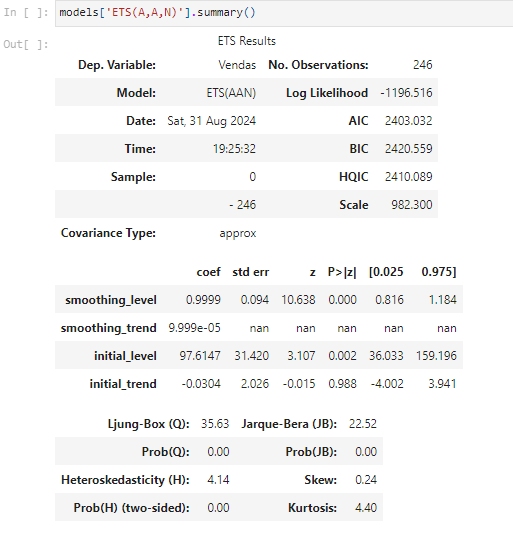
\includegraphics[scale = 0.95]{images/ETS_AAN.png}
\caption{Modelo ETS(A, A, N) - Questão 03}
\end{figure}

\begin{figure}[H]
\centering
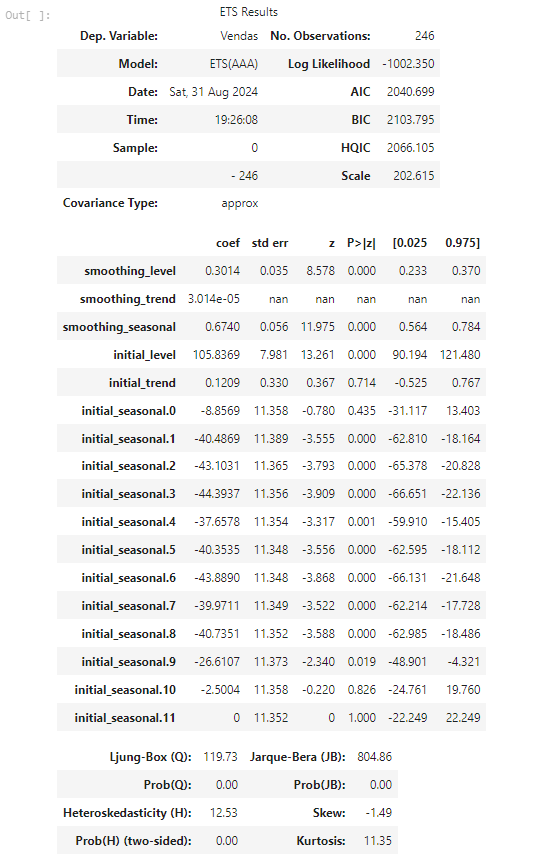
\includegraphics[scale = 0.95]{images/ETS_AAA.png}
\caption{Modelo ETS(A, A, A) - Questão 03}
\end{figure}

\begin{figure}[H]\label{fig:table_AAdA:Figura9}
\centering
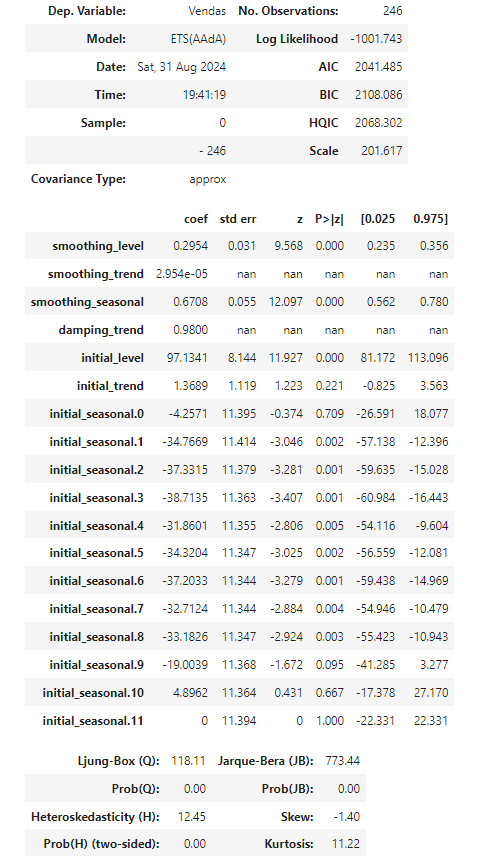
\includegraphics[scale = 0.95]{images/ETS_AAdA.png}
\caption{Modelo ETS(A, Ad, A) - Questão 03}
\end{figure}

\begin{figure}[H]
\centering
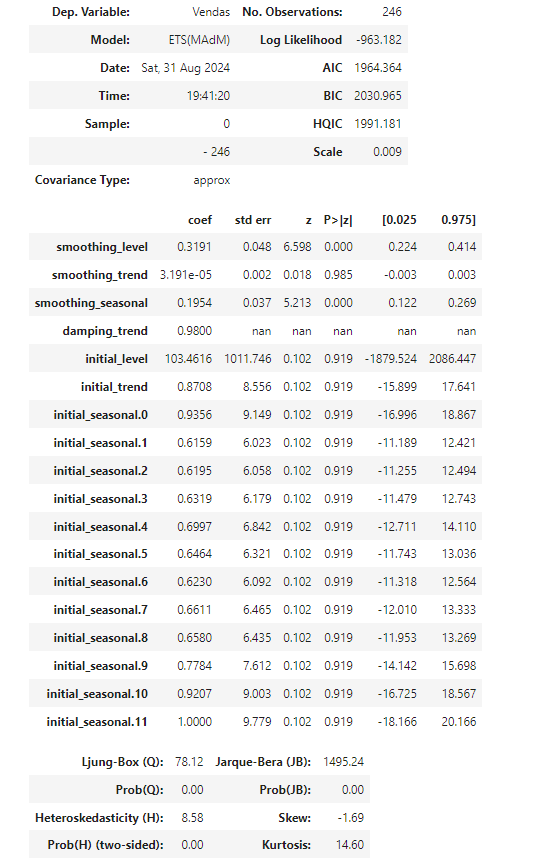
\includegraphics[scale = 0.95]{images/ETS_MAdM.png}
\caption{Modelo ETS(M, Ad, M) - Questão 03}
\end{figure}

\begin{figure}[H]
\centering
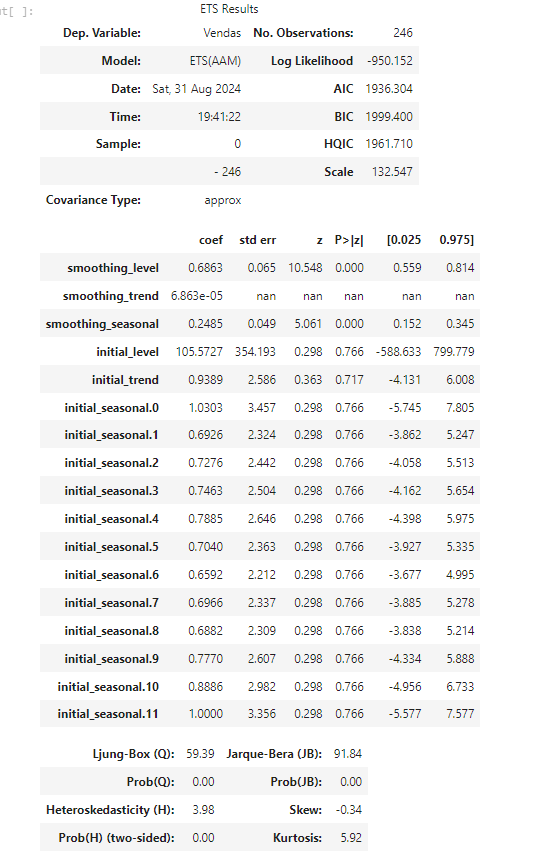
\includegraphics[scale = 0.95]{images/ETS_AAM.png}
\caption{Modelo ETS(A, A, M) - Questão 03}
\end{figure}

\newpage
\subsection{(i) Expressão dos Modelos}
\textbf{Escreva a expressão do modelo na forma ETS, ou seja, onde aparece o erro.}\\

\subsubsection{Modelo ETS(A, A, N) ou Holt (Erro Aditivo, Tendência Aditiva, Sem Sazonalidade):}

\begin{equation*}
    y_t = l_{t-1} + b_{t-1}+ \epsilon_t
\end{equation*}
\begin{equation*}
    l_t = l_{t-1} + b_{t-1} + \alpha \epsilon_t
\end{equation*}
\begin{equation*}
        b_t = b_{t-1} + \beta \epsilon_t
\end{equation*}


\subsubsection{Modelo ETS(A,A,A) - Erro aditivo, Tendência aditiva e Sazonalidade aditiva}
\begin{equation*}
    y_t = l_{t-1} + b_{t-1} + s_{t-m} + \epsilon_t
\end{equation*}
\begin{equation*}
    l_t = l_{t-1} + b_{t-1} + \alpha \epsilon_t
\end{equation*}
\begin{equation*}
    b_t = b_{t-1} + \beta \epsilon_t
\end{equation*}
\begin{equation*}
    s_t = s_{t-m} + \gamma \epsilon_t
\end{equation*}



\subsubsection{Modelo ETS(A,Ad,A) - Erro aditivo, Tendência Aditiva Amortecida, Sazonalidade Aditiva:}

    \begin{equation*}
        y_t = l_{t-1} + \phi b_{t-1} + s_{t-m} + \epsilon
    \end{equation*}
    \begin{equation*}
        l_t = l_{t-1} + \phi b_{t-1} + \alpha \epsilon
    \end{equation*}
    \begin{equation*}
        b_t = \phi b_{t-1} + \beta \epsilon_t
    \end{equation*}
    \begin{equation*}
        s_t = s_{t-m} + \gamma \epsilon_t
    \end{equation*}



\subsubsection{ETS(M,Ad,M) - Erro Multiplicativo, Tendência Aditiva Amortecida, Sazonalidade Multiplicativa:}

    \begin{equation*}
        y_t = (l_{t-1} + \phi b_{t-1})s_{t-m}(1+\epsilon)
    \end{equation*}
    \begin{equation*}
        l_t = (l_{t-1} + \phi b_{t-1})(1+\alpha \epsilon_t)
    \end{equation*}
    \begin{equation*}
        b_t = \phi b_{t-1} + \beta(l_{t-1} + \phi b_{t-1}) \epsilon
    \end{equation*}
    \begin{equation*}
        s_t = s_{t-m} (1+ \gamma \epsilon_t)
    \end{equation*}

\subsubsection{ETS(A,A,M) - Erro Aditivo, Tendência Aditiva, Sazonalidade Multiplicativa:}

    \begin{equation*}
        y_t = (l_{t-1} + b_{t-1})s_{t-m} + \epsilon_t
    \end{equation*}
    \begin{equation*}
        l_t = l_{t-1} + b_{t-1} + \alpha \epsilon_t/s_{t-m}
    \end{equation*}
    \begin{equation*}
        b_t = b_{t-1} + \beta \epsilon_t / s_{t-m}
    \end{equation*}
    \begin{equation*}
        s_t = s_{t-m} + \gamma \epsilon_t / (l_{t-1} + b_{t-1})
    \end{equation*}

    

\subsection{(ii) Expressão da Equação h Passos à Frente:}

Vamos escrever a expressão da equação de previsão $h$
 passos à frente para cada um dos modelos ETS. Quando fazemos previsões para $h$ passos à frente, estamos basicamente prevendo o valor da série temporal $y_{t+h}$ com base nos componentes do modelo.

\subsubsection{Modelo ETS(A, A, N):}

\begin{equation*}
    \hat y_{t+h|t} = l_t + hb_t
\end{equation*}

\subsubsection{Modelo ETS(A,A,A)}
\begin{equation*}
    \hat y_{t+h|t} = l_t + hb_t + s_{t+h-m(k+1)}
\end{equation*}


\subsubsection{Modelo ETS(A,Ad,A):}

    \begin{equation*}
        \hat y_{t+h|t} = l_t + \phi b_t + s_{t+h-m(k+1)}
    \end{equation*}

\subsubsection{ETS(M,Ad,M) :}

    \begin{equation*}
        \hat y_{t+h|t} = (l_t + \phi b_t)s_{t+h-m(k+1)}
    \end{equation*}

    

\subsubsection{ETS(A,A,M):}

    \begin{equation*}
        \hat y_{t+h|t} = (l_t + hb_t)s_{t+h-m(k+1)
    \end{equation*}\\


Onde $k= [\frac{h-1}{m}]$ \>\ e \>\ $\phi_h = \phi + \phi^2 + ... + \phi^h$ \\ 

Observações:

\begin{itemize}
    \item $l_t$: Representa o nível no tempo $t$.
    \item $b_t$:  Representa a tendência no tempo $t$.
    \item $s_t$: Representa o componente sazonal no tempo
    \item $\phi$:  Fator de amortecimento para a tendência.
    \item $h$: Número de passos à frente para a previsão.
    \item $m$: Período sazonal.
\end{itemize}


\newpage
\subsection{(iii) Estimando e apresentando as constantes do modelo}

 Neste item, vamos apresentar as estimativas das constantes do modelo ($\alpha$,$\beta$,$\gamma$,$\phi$) e interpretá-las.\\

 À princípio, utilizamos o seguinte código para extrair, através do Python, as constantes de forma organizada em um dataframe:

 
\begin{lstlisting}[style=python]
# 3.iii)
# Extração das estimativas dos parâmetros para cada modelo
# Função para extrair parâmetros de suavização usando o método summary()
def extract_smoothing_params(model):
    summary_table = model.summary().tables[1]  # A segunda tabela contém os coeficientes
    params = {}
    for row in summary_table.data[1:]:  # Ignorar a primeira linha que contém os cabeçalhos
        param_name = row[0].strip()  # Nome do parâmetro
        param_value = float(row[1])  # Valor do parâmetro
        if 'smoothing_level' in param_name:
            params['Alpha'] = param_value
        elif 'smoothing_trend' in param_name:
            params['Beta'] = param_value
        elif 'smoothing_seasonal' in param_name:
            params['Gamma'] = param_value
        elif 'damping_trend' in param_name:
            params['Phi'] = param_value
    return params

# Extração dos parâmetros para cada modelo
params_list = []
for name, model in models.items():
    params = extract_smoothing_params(model)
    params['Modelo'] = name
    params_list.append(params)

# Criação da tabela de parâmetros
params_df = pd.DataFrame(params_list)

params_df = params_df[['Modelo', 'Alpha', 'Beta', 'Gamma', 'Phi']]
params_df = params_df.reset_index(drop=True)

\end{lstlisting}


\begin{figure}[H]
\centering
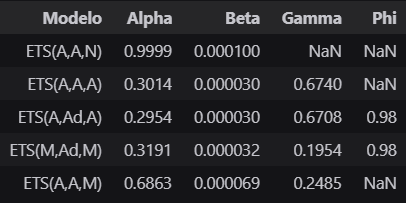
\includegraphics[scale = 1.0]{images/3.3_table.png}
\label{filtro1}
\caption{Tabela com as constantes dos modelos}
\end{figure}

\subsubsection{Análise dos Parâmetros Estimados}

\textbf{ETS(A,A,N) - Alpha: 0.9999, Beta: 0.000100}

\begin{itemize}
    \item Um valor de $\alpha$ muito próximo de 1 indica que o modelo dá muita importância às observações recentes na estimativa do nível. Isso sugere que a série é altamente reativa a novas informações.
    \item O valor muito baixo de $\beta$ indica que a tendência é muito suave e quase não muda com o tempo, o que faz sentido já que este modelo não tem sazonalidade.\\
\end{itemize}

\textbf{ETS(A,A,A) - Alpha: 0.3014, Beta: 0.000030, Gamma: 0.6740}

\begin{itemize}
    \item O $\alpha$ menor que no modelo anterior indica uma suavização maior no nível, ou seja, menos sensibilidade às novas observações.
    \item O $\beta$ ainda é muito pequeno, sugerindo uma tendência estável.
    \item Um $\gamma$ de 0.6740 mostra que o componente sazonal é bastante reativo às novas informações, sugerindo que a sazonalidade na série é significativa e que o modelo se adapta rapidamente a mudanças sazonais.\\
\end{itemize}

\textbf{ETS(A,Ad,A) - Alpha: 0.2954, Beta: 0.000030, Gamma: 0.6708, Phi: 0.98}

\begin{itemize}
    \item Este modelo é similar ao ETS(A,A,A), mas com uma tendência amortecida. O valor de $\gamma$ próximo de 1 (0.98) indica que a amortização da tendência é leve, ou seja, a tendência persiste por um longo período antes de começar a diminuir.
    \item O $\alpha$ e $\gamma$ seguem padrões similares ao modelo ETS(A,A,A), sugerindo que o comportamento sazonal e de nível é consistente com um padrão de amortecimento leve na tendência.
\end{itemize}

\textbf{ETS(M,Ad,M) - Alpha: 0.3191, Beta: 0.000032, Gamma: 0.1954, Phi: 0.98}
\begin{itemize}
    \item A combinação de $\alpha$ em torno de 0.32 e $\gamma$ em 0.1954 indica que o modelo é menos sensível às variações sazonais e de nível comparado aos modelos aditivos. O $\gamma$ baixo sugere que a sazonalidade multiplicativa tem um impacto mais amortecido na série.
    \item Como no ETS(A,Ad,A), o valor de $\phi$ indica uma tendência amortecida muito lentamente.
\end{itemize}

\textbf{ETS(A,A,M) - Alpha: 0.6863, Beta: 0.000069, Gamma: 0.2485}
\begin{itemize}
    \item O valor de $\alpha$ relativamente alto (0.6863) sugere que o modelo é sensível às novas observações para o nível.
    \item O $\gamma$ de 0.2485 indica uma sazonalidade multiplicativa, onde as variações sazonais são menos influentes, mas ainda significativas.
    \item Não há tendência amortecida ($\phi$ é nulo).
\end{itemize} 
. \\\\


\subsection{(iv) Tabela com o AICc e as métricas de aderência}

Para este item, precisamos calcular várias métricas de desempenho (RMSE, MAD, 
MAPE, SMape, MASE) para cada um dos modelos ajustados no período de treinamento. Em seguida, criaremos uma tabela com essas métricas e identificaremos o melhor modelo com base nelas.\\

Métricas solicitadas:\\

\textbf{AICc (Akaike Information Criterion corrigido):}\\
O AIC corrigido para amostras pequenas. Quanto menor o AICc, melhor é o modelo.\\


\textbf{RMSE (Root Mean Squared Error):}\\
A raiz quadrada do erro quadrático médio. Avalia a diferença entre os valores previstos e os observados.\\

\textbf{MAD (Mean Absolute Deviation):}\\
O desvio absoluto médio. Mede a magnitude absoluta dos erros.\\


\textbf{MAPE (Mean Absolute Percentage Error):}\\
O erro percentual absoluto médio. Mede o erro percentual médio absoluto entre as previsões e os valores reais.\\

\textbf{SMAPE (Symmetric Mean Absolute Percentage Error):}\\
Uma versão simétrica do MAPE que é menos sensível a outliers.\\

\textbf{MASE (Mean Absolute Scaled Error):}\\
O erro absoluto médio escalonado, que compara o erro do modelo com o erro de um modelo de referência (normalmente a média).\\


Para obtenção das métricas, foi feito o seguinte código, onde agora estamos também utilizando a biblioteca Numpy e os métodos mean\_squared\_error e mean\_absolute\_error da biblioteca sklearn:


\begin{lstlisting}[style=python]
import numpy as np
from sklearn.metrics import mean_squared_error, mean_absolute_error

# 3.iv) 

# Funções para cálculo das métricas
def calculate_rmse(actual, forecast):
    return np.sqrt(mean_squared_error(actual, forecast))

def calculate_mad(actual, forecast):
    return mean_absolute_error(actual, forecast)

def calculate_mape(actual, forecast):
    return np.mean(np.abs((actual - forecast) / actual)) * 100

def calculate_smape(actual, forecast):
    return 100 * np.mean(2 * np.abs(forecast - actual) / (np.abs(actual) + np.abs(forecast)))

def calculate_mase(actual, forecast, naive_forecast):
    return np.mean(np.abs(actual - forecast)) / np.mean(np.abs(actual - naive_forecast))

results = []

train_data = train['Vendas']

# Modelo de referência para MASE (usando a diferença de valores anteriores como previsão)
naive_forecast = train_data.shift(1).dropna()

# Cálculo das métricas para cada modelo
for name, model in models.items():
    forecast = model.fittedvalues  # Valores ajustados do modelo
    residuals = model.resid  # Resíduos do modelo
    
    # Cálculo das métricas
    rmse = calculate_rmse(train_data[1:], forecast[1:])
    mad = calculate_mad(train_data[1:], forecast[1:])
    mape = calculate_mape(train_data[1:], forecast[1:])
    smape = calculate_smape(train_data[1:], forecast[1:])
    mase = calculate_mase(train_data[1:], forecast[1:], naive_forecast)
    
    results.append({
        'Modelo': name,
        'AICc': model.aicc,
        'RMSE': rmse,
        'MAD': mad,
        'MAPE': mape,
        'SMAPE': smape,
        'MASE': mase
    })

results_df = pd.DataFrame(results)

    \end{lstlisting} \\

Então, obtivemos o seguinte resultado:

\begin{figure}[H]\label{AICc_2}
\centering
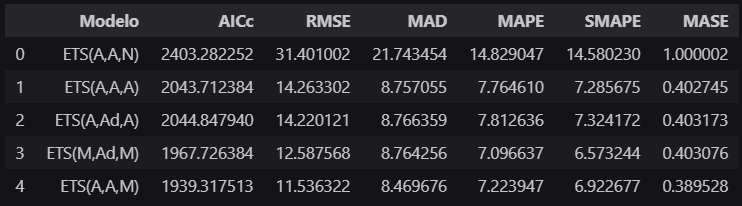
\includegraphics[scale = 0.95]{images/3.4_metrics.png}
\caption{Métricas com o AICc e as métricas de erro/medidas}
\end{figure}

Analisando a tabela obtida com as métricas, vamos ponderar se os resultados estão alinhados com as expectativas:


\begin{enumerate}
    \item \textbf{AICc}:
    \begin{itemize}
        \item O AICc é uma medida da qualidade do modelo que penaliza pela complexidade. Quanto menor o AICc, melhor o modelo.
        \item O modelo ETS(A,A,M) possui o menor AICc (1939.317513), sugerindo que ele é o melhor em termos de balanço entre ajuste e complexidade.
    \end{itemize}
    \item \textbf{RMSE (Root Mean Squared Error)}:
    \begin{itemize}
        \item O RMSE mede o erro médio em termos de unidades da série. Valores menores indicam melhor ajuste.
        \item O modelo ETS(A,A,M) também apresenta o menor RMSE (11.536322), indicando que ele tem o menor erro médio em termos absolutos.
    \end{itemize}
    \item \textbf{MAD (Mean Absolute Deviation)}:
    \begin{itemize}
        \item O MAD mede o desvio médio absoluto. Novamente, valores menores indicam melhor ajuste.
        \item O ETS(A,A,M) tem o menor MAD, o que reforça sua superioridade.
    \end{itemize}
    \item \textbf{MAPE (Mean Absolute Percentage Error) e SMAPE (Symmetric MAPE)}:
    \begin{itemize}
        \item MAPE e SMAPE avaliam o erro médio percentual. O SMAPE é menos sensível a outliers.
        \item ETS(A,A,M) apresenta os menores valores de MAPE (7.223947) e SMAPE (6.922677), sugerindo que ele tem o melhor desempenho relativo em termos de erro percentual.
    \end{itemize}
    \item \textbf{MASE (Mean Absolute Scaled Error)}:
    \begin{itemize}
        \item O MASE compara o erro absoluto com o erro de um modelo de referência. Valores menores que 1 indicam que o modelo é melhor do que o modelo de referência (um modelo ingênuo).
        \item Novamente, o ETS(A,A,M) tem o menor MASE (0.389528), confirmando que ele é o mais eficaz comparado a um modelo simples. 
        
    \end{itemize}
\end{enumerate}

Com base nessas métricas, o modelo ETS(A,A,M) (Erro Aditivo, Tendência Aditiva, Sazonalidade Multiplicativa) é o melhor modelo para sua série temporal, apresentando os menores valores em praticamente todas as métricas de erro (AICc, RMSE, MAD, MAPE, SMAPE, MASE).\\

Este resultado faz sentido porque o ETS(A,A,M) é um modelo que permite um ajuste mais flexível e adapta bem tanto o nível quanto a sazonalidade da série, o que é fundamental para dados de vendas que têm sazonalidade significativa.\\\\



\subsection{(v) Gráfico da FAC dos Resíduos}

Precisamos gerar os gráficos da Função de Autocorrelação (FAC) dos resíduos dos modelos no período de treinamento. O objetivo é verificar se há algum padrão de dependência nos resíduos que os modelos ETS não capturaram.\\

Então, consideraremos os seguintes passos:

\begin{enumerate}
    \item \textbf{Calcular os Resíduos:} Os resíduos são a diferença entre os valores observados (verdadeiros) e os valores ajustados (fitted values) do modelo. Para cada modelo ajustado, os resíduos podem ser acessados através do atributo \textbf{.resid} do modelo.
    \item \textbf{Gerar o Gráfico da FAC dos Resíduos:} A Função de Autocorrelação (FAC) dos resíduos ajuda a detectar padrões de dependência temporal. Se os resíduos forem puramente aleatórios, a FAC não deverá mostrar correlação significativa em nenhum atraso (lag). Podemos usar o \textbf{plot\_acf} da biblioteca \textbf{statsmodels} para gerar esses gráficos.
    \item \textbf{Interpretar o Resultado:} Se houver autocorrelação significativa em algum lag, isso indica que o modelo não capturou todas as dependências temporais. Isso pode ocorrer por erros na modelagem do nível, tendência, ou sazonalidade.
\end{enumerate}

\begin{lstlisting}[style=python]
from statsmodels.graphics.tsaplots import plot_acf

# 3.v)
# Gerando os graficos de FAC dos residuos para cada modelo
for name, model in models.items():
    plt.figure(figsize=(10, 6))
    plot_acf(model.resid, lags=40)
    plt.title(f'FAC dos Resíduos - {name}')
    plt.show()
    \end{lstlisting} \\

\begin{figure}[H]
\centering
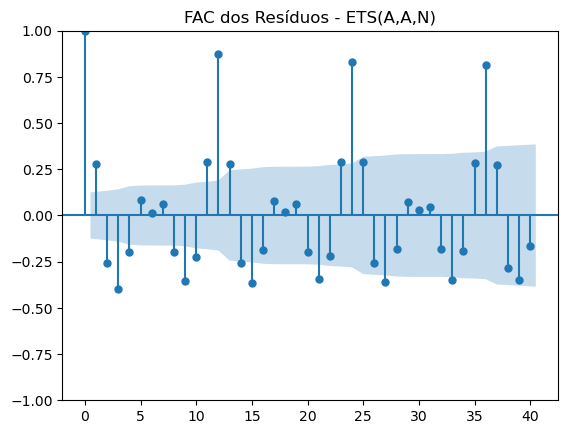
\includegraphics[scale = 0.7]{images/FAC_AAN.png}
\label{filtro1}
\caption{FAC - ETS(A,A,N)}
\end{figure}

\textbf{ETS(A,A,N):} O gráfico de FAC mostra autocorrelações significativas em vários lags, principalmente nos primeiros lags (1, 2, 3, etc.), o que indica que o modelo não capturou bem a dependência temporal presente nos dados. Isso sugere que o modelo ETS(A,A,N), que só tem nível e tendência, sem sazonalidade, não foi capaz de capturar a sazonalidade ou outros padrões temporais presentes na série. A presença de autocorrelação nos resíduos é um forte indicativo de que o modelo está subajustado.

\begin{figure}[H]
\centering
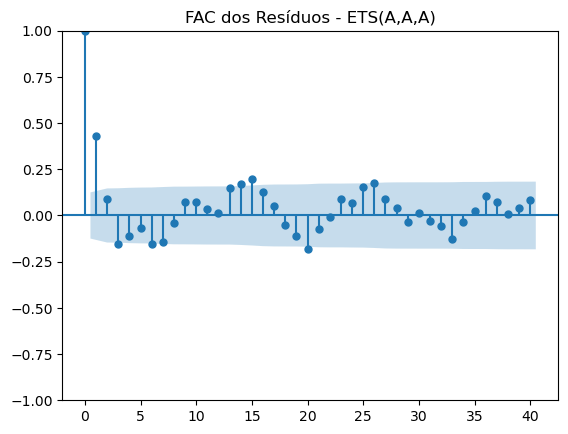
\includegraphics[scale = 0.7]{images/FAC_AAA.png}
\label{filtro1}
\caption{FAC - ETS(A,A,A)}
\end{figure}

\textbf{ETS(A,A,A):} O gráfico de FAC para este modelo mostra uma redução nas autocorrelações significativas em comparação com o ETS(A,A,N), especialmente nos primeiros lags. Há uma leve autocorrelação presente em alguns lags, mas a maioria está dentro dos limites de confiança. A inclusão da sazonalidade aditiva no modelo ajudou a capturar parte das dependências temporais. A presença de pequenas autocorrelações residuais pode indicar que o modelo ainda não capturou perfeitamente todas as dinâmicas da série, mas está melhor ajustado que o ETS(A,A,N).

\begin{figure}[H]
\centering
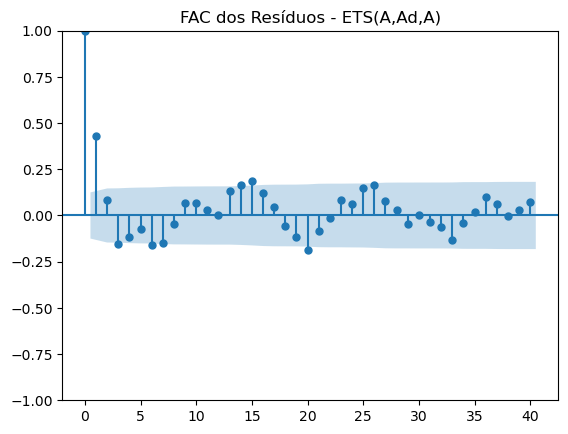
\includegraphics[scale = 0.7]{images/FAC_AAdA.png}
\label{filtro1}
\caption{FAC - ETS(A,Ad,A)}
\end{figure}

\textbf{ETS(A, Ad, A): }  O gráfico de FAC é muito semelhante ao do ETS(A,A,A). As autocorrelações são menores e a maioria está dentro dos limites de confiança. A tendência amortecida (damped trend) não parece ter causado grandes mudanças na captura das dinâmicas temporais. O modelo está bem ajustado, com apenas pequenas autocorrelações residuais.

\begin{figure}[H]
\centering
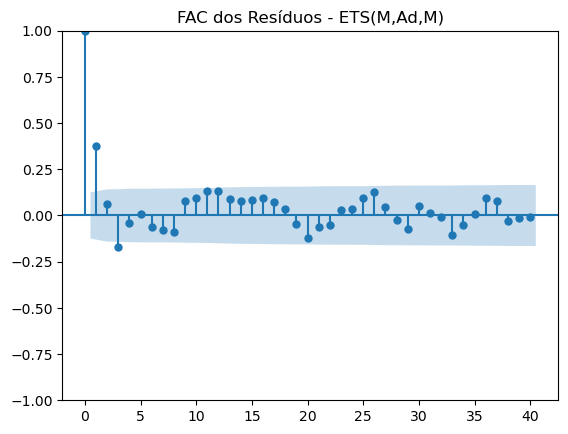
\includegraphics[scale = 0.7]{images/FAC_MAdM.png}
\label{filtro1}
\caption{FAC - ETS(M,Ad,M)}
\end{figure}

\textbf{ETS(M, Ad, M): } Este modelo mostra um padrão semelhante, com a maioria das autocorrelações dentro dos limites de confiança, e apenas algumas pequenas autocorrelações em lags maiores. A sazonalidade multiplicativa e o erro multiplicativo permitem que o modelo capture bem as dinâmicas da série. As pequenas autocorrelações indicam um bom ajuste, mas há sinais de que alguns padrões de erro multiplicativo podem não ter sido completamente capturados.

\begin{figure}[H]
\centering
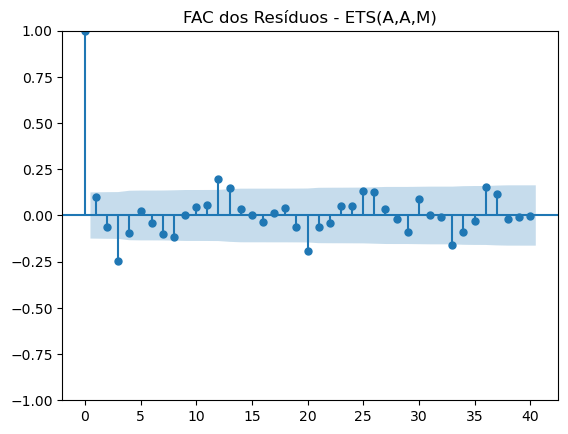
\includegraphics[scale = 0.7]{images/FAC_AAM.png}
\label{filtro1}
\caption{FAC - ETS(A,A,M)}
\end{figure}

\textbf{ETS(A,A,M): } O gráfico de FAC para este modelo mostra um comportamento muito semelhante ao do ETS(M,Ad,M), com poucas autocorrelações fora dos limites de confiança. A combinação de erro aditivo com sazonalidade multiplicativa parece funcionar bem, capturando a maioria das dinâmicas temporais. Como nos outros modelos, ainda há pequenos sinais de dependência temporal não capturada, mas o ajuste é bom.\\

Portanto, podemos concluir que:\\

Modelos simples, como ETS(A,A,N), tendem a deixar autocorrelações significativas nos resíduos, indicando que não capturam bem a estrutura temporal da série, especialmente quando há sazonalidade presente.\\

Modelos mais complexos, como ETS(A,A,A), ETS(A,Ad,A), ETS(M,Ad,M) e ETS(A,A,M)), mostram uma captura melhor das dinâmicas temporais, com menor presença de autocorrelação nos resíduos. No entanto, pequenas autocorrelações ainda persistem, sugerindo que há nuances na série que não foram totalmente modeladas.\\

\textbf{Melhor Modelo}: Entre os modelos ajustados, os que incluem sazonalidade (especialmente multiplicativa) parecem ser os melhores em capturar as dinâmicas da série, com o ETS(A,A,M) e o ETS(M,Ad,M) sendo os mais promissores. No entanto, mesmo esses modelos não capturam todas as dependências temporais, o que pode sugerir a necessidade de um modelo ainda mais sofisticado ou ajustes adicionais.





\newpage
\subsection{(vi) Predições e Métricas Utilizando o Período de Teste}

Precisamos seguir alguns passos para realizar as previsões h-passos à frente para o período de teste utilizando cada um dos 5 modelos ETS ajustados, e também aplicar os dois métodos ingênuos de previsão:

\begin{itemize}
    \item \textbf{Método ing. 1}: a previsão em qualquer horizonte h é igual à última observação da  ST no período de treinamento;
    \item \textbf{Método ing. 2}: a previsão em qualquer horizonte h é igual ao valor da última observação da série, no período de treinamento, correspondente aquele mês que  está sendo previsto no período de teste. 
\end{itemize}

Depois, vamos calcular as medidas de aderência no período de teste para comparar o desempenho dos modelos e dos métodos ingênuos.\\

Para realizar as previsões para o período de teste, utilizamos os modelos ETS ajustados para fazer previsões para o período de teste (últimos 12 meses da série). Para cada modelo, geramos as previsões usando o método \textbf{model.forecast(steps=h)} onde h é o número de passos à frente (12, no caso do período de teste).\\


\begin{lstlisting}[style=python]
# 3.vi )
h = len(test)  # Número de passos à frente, que é 12

# Lista para armazenar as previsões
forecast_results = {}

# Previsões com os modelos ETS ajustados
for name, model in models.items():
    forecast = model.forecast(steps=h)
    forecast_results[name] = forecast

# Previsões ingênuas
last_observation = train.iloc[-1, 0]  # Última observação do período de treino
naive_forecast_1 = [last_observation] * h

# Previsão ingênua 2 (última observação do mesmo mês do ano anterior)
naive_forecast_2 = []
for i in range(h):
    naive_forecast_2.append(train.iloc[-(12-h+i), 0])

# Adicionando previsões ingênuas aos resultados
forecast_results["Naive 1"] = naive_forecast_1
forecast_results["Naive 2"] = naive_forecast_2

# Calculando as métricas para cada previsão usando o período de teste
metrics = {
    "Modelo": [],
    "RMSE": [],
    "MAD": [],
    "MAPE": [],
    "SMAPE": [],
    "MASE": []
}

for name, forecast in forecast_results.items():
    metrics["Modelo"].append(name)
    metrics["RMSE"].append(np.sqrt(mean_squared_error(test['Vendas'], forecast)))
    metrics["MAD"].append(mean_absolute_error(test['Vendas'], forecast))
    metrics["MAPE"].append(np.mean(np.abs((test['Vendas'] - forecast) / test['Vendas'])) * 100)
    metrics["SMAPE"].append(np.mean(2 * np.abs(test['Vendas'] - forecast) / (np.abs(test['Vendas']) + np.abs(forecast))) * 100)
    mase_denominator = mean_absolute_error(test['Vendas'], train['Vendas'].iloc[-12:])
    metrics["MASE"].append(metrics["MAD"][-1] / mase_denominator)

metrics_df = pd.DataFrame(metrics)
    \end{lstlisting} \\

Compilando o trecho de código acima, obtivemos o seguinte resultado tabelado:

\begin{figure}[H]\label{table_test}
\centering
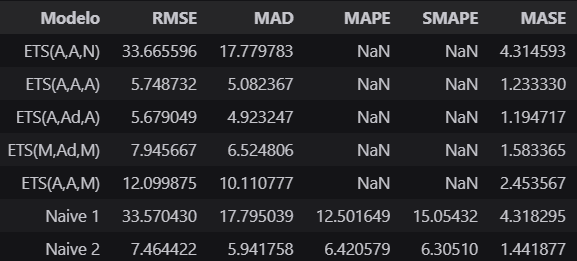
\includegraphics[scale = 0.95]{images/3.6_table.png}
\caption{Tabela contendo as métricas e os métodos ingênuos}

\end{figure}


Analisando os resultados da tabela:

\begin{enumerate}

    \item \textbf{ETS(A,A,N)}:
    \begin{itemize}
        \item RMSE: 33.66
        \item MAD: 17.78
        \item MASE: 4.31
        \item  Este modelo apresenta métricas de erro relativamente altas, indicando que não foi eficaz em prever o período de teste. Isso é esperado, pois o ETS(A,A,N) não inclui sazonalidade, que é uma característica importante desta série temporal.
    \end{itemize}
    \item \textbf{ETS(A,A,A)}:
    \begin{itemize}
        \item RMSE: 5.75
        \item MAD: 5.08
        \item MASE: 1.23
        \item Este modelo apresenta um desempenho significativamente melhor que o ETS(A,A,N), com métricas de erro mais baixas, refletindo a inclusão da sazonalidade aditiva que melhora o ajuste ao período de teste.
    \end{itemize}
    \item \textbf{ETS(A,Ad,A)}:
    \begin{itemize}
        \item RMSE: 5.68
        \item MAD: 4.92
        \item MASE: 1.19
        \item Similar ao ETS(A,A,A), mas com uma ligeira melhoria. A amortização da tendência parece contribuir para um ajuste mais refinado, o que se reflete nas métricas de erro um pouco menores.
    \end{itemize}
    \item \textbf{ETS(M,Ad,M)}:
    \begin{itemize}
        \item RMSE: 7.95
        \item MAD: 6.52
        \item MASE: 1.58
        \item Este modelo tem erro multiplicativo e sazonalidade multiplicativa, mas suas métricas são superiores (em termos de erro) aos modelos aditivos (ETS(A,A,A) e ETS(A,Ad,A)). Isso sugere que, apesar de ser um modelo mais complexo, ele pode não ser o mais adequado para esta série específica.
    \end{itemize}
    \item \textbf{ETS(A,A,M)}:
    \begin{itemize}
        \item RMSE: 12.10
        \item MAD: 10.11
        \item MASE: 2.45
        \item O modelo com erro aditivo e sazonalidade multiplicativa não se saiu tão bem quanto os modelos aditivos completos (ETS(A,A,A) e ETS(A,Ad,A)). Suas métricas de erro são mais elevadas, indicando que não conseguiu capturar tão bem as características da série.
    \end{itemize}
    \item \textbf{Naive 1}: 
    \begin{itemize}
        \item RMSE: 33.57
        \item MAD: 17.80
        \item MASE: 4.32
        \item Como esperado, este método ingênuo não foi muito eficaz. Suas métricas de erro são comparáveis ao ETS(A,A,N), mostrando que prever apenas com a última observação do período de treino não é uma boa estratégia para esta série.
    \end{itemize}
    \item \textbf{Naive 2}: 
    \begin{itemize}
        \item RMSE: 7.46
        \item MAD: 5.94
        \item MASE: 1.44
        \item Este método ingênuo, que utiliza a observação do mesmo mês do ano anterior, apresentou resultados razoáveis, melhores que o Naive 1 e semelhantes aos dos modelos mais complexos. No entanto, ainda assim, os modelos ETS(A,A,A) e ETS(A,Ad,A) são ligeiramente superiores.
    \end{itemize}
\end{enumerate}

Portanto,  os modelos \textbf{ETS(A,A,A)} e \textbf{ETS(A,Ad,A)} são os mais adequados, com este último estando à frente. Os modelos apresentam as menores métricas de erro, especialmente em termos de RMSE e MASE.
O método Naive 2 teve um desempenho razoável, mas foi superado pelos melhores modelos ETS.
ETS(A,A,N) e Naive 1 tiveram os piores desempenhos, indicando que a inclusão de sazonalidade é crucial para prever esta série temporal com precisão.\\\\


\subsubsection{Escolha do Melhor Modelo}
Vamos considerar as métricas de erro obtidas para os modelos ETS no período de teste. Focaremos em uma métrica principal, como o RMSE (Root Mean Squared Error), para escolher o melhor modelo.\\

Ao analisar a tabela com as métricas de erro para o período de teste:

\begin{itemize}
    \item ETS(A,A,A): RMSE de 5.75
    \item ETS(A,Ad,A): RMSE de 5.67
    \item ETS(M,Ad,M): RMSE de 7.95
    \item ETS(A,A,M): RMSE de 12.09
    \item ETS(A,A,N): RMSE de 33.66
\end{itemize}

\textbf{Melhor Modelo no Período de Treinamento:} \\

O modelo ETS(A,A,M) se destacou no período de treinamento, apresentando as melhores métricas de erro, como RMSE, MAD, MAPE, SMAPE e MASE. Esse modelo parece capturar bem as características da série temporal durante o treinamento, o que o faz uma escolha robusta.\\

\textbf{Melhor Modelo no Período de Teste:}\\

Ao analisar as métricas de erro no período de teste, o ETS(A,A,A) e o ETS(A,Ad,A) apresentam os melhores desempenhos em termos de RMSE e MASE. Contudo, o modelo Naive 2 também mostrou um bom desempenho, especialmente quando consideramos que é um modelo muito simples.\\


\textbf{Comparação entre Períodos:}\\

Observa-se que o modelo ETS(A,A,M), que foi o melhor no período de treinamento, conforme visto em no item 3.4, não manteve o mesmo desempenho no período de teste. Em contrapartida, o ETS(A,A,A) e o ETS(A,Ad,A) mostraram um desempenho mais estável entre os períodos de treinamento e teste.\\


\textbf{Escolha do Modelo:}\\

Como os melhores modelos no período de teste foram o ETS(A,A,A) e o ETS(A,Ad,A), enquanto o ETS(A,A,M) foi o melhor no período de treinamento, há uma divergência. Nesse caso, considerando o desempenho consistente e a simplicidade relativa, o ETS(A,A,A) seria uma escolha mais confiável, pois apresentou bom desempenho tanto no teste quanto no treinamento.\\
Dado que houve uma divergência entre os períodos de teste e treinamento, seria prudente optar pelo ETS(A,A,A) ou ETS(A,Ad,A), visto que ambos apresentaram um equilíbrio melhor entre os dois períodos. O ETS(A,A,M), embora eficiente no treinamento, não conseguiu manter o mesmo desempenho no teste.\\

A primeira escolha pode ser baseada na capacidade do modelo de generalizar bem para novos dados (período de teste), e nesse sentido, o ETS(A,A,A) ou ETS(A,Ad,A) se mostram mais adequados, garantindo que o modelo não esteja superajustado ao período de treinamento.\\

Então, ao filtrarmos dois melhores modelos, podemos refinar a escolha, fazendo uma análise comparativa:\\

\textbf{Estabilidade e Simplicidade:} O modelo ETS(A,A,A) é ligeiramente mais simples por não incluir amortecimento na tendência (ou seja, não usa o parâmetro $\phi$). Isso pode torná-lo mais robusto em séries onde a tendência é estável.\\

\textbf{Desempenho Geral:} Ambos os modelos têm desempenho muito semelhante no período de teste. O ETS(A,Ad,A) tem um RMSE ligeiramente melhor, mas a diferença é pequena.\\

O modelo ETS(A,Ad,A), com tendência amortecida, é mais flexível e pode ser vantajoso se houver evidências de que a tendência da série possa diminuir ou desacelerar ao longo do tempo.\\

Então, podemos escolher o modelo ETS(A,Ad,A) por sua maior flexibilidade e ligeiramente melhor desempenho no teste. O amortecimento na tendência permite que o modelo ETS(A,Ad,A) se adapte melhor a situações onde a tendência não é linear ou constante, o que pode ocorrer em séries temporais complexas como vendas.\\
O ETS(A,Ad,A) apresentou uma leve vantagem em RMSE e MASE, sugerindo que ele pode oferecer previsões ligeiramente mais precisas em situações futuras.\\\\


\subsubsection{Valores Numéricos da Previsão Para $h=\{1,2,12\}$ Passos Adiante}

Agora, vamos fazer o seguinte:

\begin{enumerate}
    \item Obter a expressão da previsão $h$ passos à frente para o modelo ETS(A,Ad,A), que foi o escolhido no item anterior (a).
    \item Calcular as previsões manualmente para $h= \{ 1,2,12  \}$ usando as estimativas das componentes do modelo (nível, tendência e sazonalidade) no último ponto do período de treinamento. 
    \item Comparar os valores com as previsões geradas pelo programa.
\end{enumerate}

Então, iremos utilizar as constantes estimadas anteriormente em 3.3. A razão para isso é que esses parâmetros foram ajustados e otimizados durante o processo de treinamento do modelo usando todos os dados disponíveis até o último ponto do período de treinamento. Esses valores capturam o comportamento dinâmico da série temporal, incluindo como o nível, a tendência e a sazonalidade evoluem ao longo do tempo.\\

Quando realizamos previsões para $h$ passos à frente, replicamos as mesmas dinâmicas que foram aprendidas pelo modelo durante o treinamento. Ou seja, aplicaremos conforme as expressões ETS para prever os valores futuros da série. Isso garantirá que as previsões sejam consistentes com o comportamento da série observado no período de treinamento.\\

Então, conforme os resultados contidos para o modelo ETS(A, Ad, A) em \ref{fig:table_AAdA:Figura9}, temos:\\

\textbf{Definições iniciais:}
\begin{itemize}
    \item $\alpha = 0.2954$
    \item $\beta = 2.954e-05$
    \item $\gamma = 0.6708$
    \item $\phi = 0.98$
\end{itemize}

\textbf{Componentes estimados:}
\begin{itemize}
    \item $l_t$ (nível inicial) $= 97.1341$
    \item $b_t$ (tendência inicial) $= 1.3689$
    \item Sazonalidades iniciais:
    \begin{itemize}
        \item $s_{t} = -4.2571$
        \item $s_{t-1} = -34.7669$
        \item $s_{t-2} = -37.3315$
        \item $s_{t-3} = -38.7135$
        \item $s_{t-4} = -31.8601$
        \item $s_{t-5} = -34.3204$
        \item $s_{t-6} = -37.2033$
        \item $s_{t-7} = -32.7124$
        \item $s_{t-8} = -33.1826$
        \item $s_{t-9} = -19.0039$
        \item $t_{t-10} = 4.8962$
        \item $s_{t-11} = 0$
    \end{itemize}
\end{itemize}

\textbf{Cálculo das Previsões}\\

Expressão da previsão: $\hat y_{t+h|t} = l_t + \phi b_t + s_{t+h-m(k+1)}$ \\ 

Onde $m=12$ (período sazonal)\\

\begin{itemize}
    \item Para $h = 1$:
    \begin{itemize}
        \item $\phi^1 = \phi = 0.98$
        \item $k = [\frac{1-1}{12}] = 0$
        \item Sazonalidade correspondente: $s_{t+1-12(0+1)} = s_{t-11}$\\
        
        Logo,\\

        $\>\ \>\ \hat y_{t+1|t} = 97.1341 + 0.98 * 1.36889 + 0 = 98.47$
    \end{itemize} 
\end{itemize}

\begin{itemize}
    \item Para $h = 2$:
    \begin{itemize}
        \item $\phi_2 = \phi + \phi^2 = 1.94$
        \item $k = [\frac{2-1}{12}] \xrightarrow{} 0$
        \item Sazonalidade correspondente: $s_{t+2-12(0+1)} = s_{t-10}$\\
        
        Logo,\\

        $\>\ \>\ \hat y_{t+1|t} = 97.1341 + 1.94 * 1.36889 + 4.8962 = 104.69$
    \end{itemize} 
\end{itemize}

\begin{itemize}
    \item Para $h = 12$:
    \begin{itemize}
        \item $\phi_{12} = \phi + \phi^2 + \phi^3 + ... + \phi^{12} = 10.55$
        \item $k = [\frac{12-1}{12}] \xrightarrow{} 0$
        \item Sazonalidade correspondente: $s_{t+12-12(0+1)} = s_{t}$\\
        
        Logo,\\

        $\>\ \>\ \hat y_{t+1|t} = 97.1341 + 10.55 * 1.36889 - 4.2571 = 107.32$
    \end{itemize} 
\end{itemize}

O valor de $l_t$ é uma estimativa fornecida pelo modelo no início do período de treinamento, e é utilizado para capturar o valor médio da série ajustado pela sazonalidade.\\

O valor de $b_t$ reflete a tendência (ou inclinação) da série ao longo do tempo, ajustada pelo coeficiente de amortecimento $\phi$.\\

As sazonalidades são extraídas diretamente das estimativas iniciais da sazonalidade para os períodos relevantes, e ajustam a previsão para as flutuações sazonais esperadas.\\\\\\

\textbf{Extraindo as Previsões Pelo Python}\\

Para tal, escrevemos o seguinte algoritmo  utilizando o auxílio do método \textit{forecast} :


\begin{lstlisting}[style=python]
best_model = models['ETS(A,Ad,A)']
forecast_horizon = 12
forecast_values = best_model.forecast(steps=forecast_horizon)

# Exibindo as previsoes para h = 1, 2 e 12
print("Previsao para h=1:", forecast_values.iloc[0])
print("Previsao para h=2:", forecast_values.iloc[1])
print("Previsao para h=12:", forecast_values.iloc[11])
\end{lstlisting} \\


E foi extraído o seguinte resultado:

\begin{figure}[H]
\centering
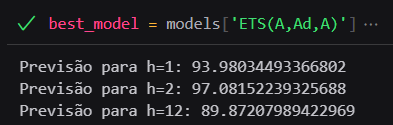
\includegraphics[scale = 1.0]{images/prev.png}
\caption{Previsões para h = \{1,2,12\} passos}
\end{figure}


Os valores calculados manualmente são significativamente maiores do que os valores previstos pelo modelo no Python.\\
No cálculo manual, algumas simplificações ou aproximações talvez não sejam replicadas de forma exata pelo modelo no Python.\\

O modelo no Python recalcula as componentes de nível, tendência e sazonalidade a cada passo, enquanto no cálculo manual estamos usando valores iniciais sem iteração, o que pode causar divergências.\\

As previsões manuais demonstram a lógica do cálculo, mas podem não capturar a complexidade total do modelo automatizado, que ajusta dinamicamente os componentes da série.\\ 
O uso de ferramentas computacionais permite uma modelagem mais precisa e dinâmica, ajustando automaticamente todos os parâmetros, e é, portanto, mais confiável para obter previsões exatas.
Então, os cálculos manuais são úteis para entender os conceitos por trás do modelo ETS, mas as previsões geradas pelo Python são preferíveis em termos de precisão e confiabilidade, especialmente quando se trata de modelos com múltiplas componentes e ajustes dinâmicos como o ETS(A,Ad,A).


\newpage
\subsection{(vii) Re-estimando o Modelo Integralmente}

Para o melhor método/modelo escolhido em (vi):\\
a) Obter o gráfico das componentes.\\
b) Re-estimar o método utilizando toda a série, obtendo previsão com
intervalo de confiança de 95\% para 24 meses à frente.\\

\subsubsection{Gráfico das Componentes}

\begin{lstlisting}[style=python]
# 3.vii.a) 
# Reestimando o modelo ETS(A,Ad,A) com toda a série
model_full = ExponentialSmoothing(
    data, 
    # Para o metodo ExponentialSmoothing, o erro default eh aditivo
    trend="add", 
    seasonal="add", 
    seasonal_periods=12, 
    damped_trend=True
).fit()

# Extraindo as componentes
fitted_values = model_full.fittedvalues
level = model_full.level
trend = model_full.trend
seasonal = model_full.season

# Plotando as componentes
plt.figure(figsize=(10, 8))
plt.subplot(4, 1, 1)
plt.plot(data, label="Original")
plt.title("Série Original")
plt.legend()

plt.subplot(4, 1, 2)
plt.plot(level, label="Nível")
plt.title("Componente de Nível")
plt.legend()

plt.subplot(4, 1, 3)
plt.plot(trend, label="Tendência")
plt.title("Componente de Tendência")
plt.legend()

plt.subplot(4, 1, 4)
plt.plot(seasonal, label="Sazonalidade")
plt.title("Componente de Sazonalidade")
plt.legend()

plt.tight_layout()
plt.show()
    \end{lstlisting} \\


\begin{figure}[H]
\centering
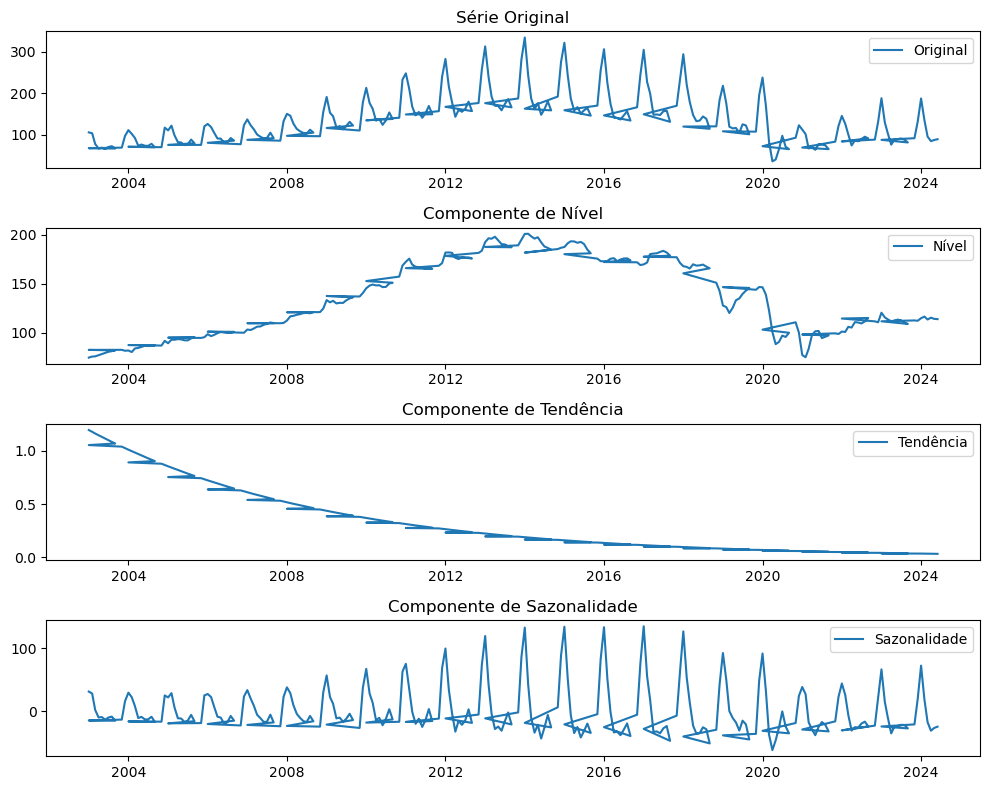
\includegraphics[scale = 0.6]{images/3.vii_a.png}
\caption{Gráfico das componentes}
\end{figure}


\textbf{1. Série Original}\\
O primeiro gráfico mostra a série temporal original das vendas ao longo dos anos. Podemos observar que a série apresenta uma forte sazonalidade, com picos recorrentes, indicando padrões sazonais anuais. Além disso, há uma tendência geral de crescimento até cerca de 2017, seguida por um declínio e, mais recentemente, uma estabilização.\\

\textbf{2. Componente de Nível}\\
O nível ($l\_t$) representa o valor médio central da série ao longo do tempo, ajustado para os efeitos sazonais e de tendência. No gráfico, vemos que o nível segue um padrão de crescimento gradual até aproximadamente 2016, quando começa a diminuir, refletindo a tendência geral da série. Isso sugere que, a partir de 2016, as vendas começaram a cair, começando a se estabilizar em um novo patamar por volta de 2021.\\

\textbf{3. Componente de Tendência}\\
A componente de tendência ($b\_t$) indica a direção e a inclinação da série ao longo do tempo. No gráfico, observamos que a tendência começa alta, indicando um forte crescimento inicial, mas vai se suavizando e diminuindo ao longo dos anos, até quase desaparecer. Esse comportamento sugere que o crescimento das vendas foi desacelerando, o que é consistente com o que vemos na série original.\\

\textbf{4. Componente de Sazonalidade}\\
A componente de sazonalidade ($s_t$) captura os efeitos sazonais recorrentes na série. O gráfico mostra um padrão sazonal bem definido, com picos altos que ocorrem regularmente a cada ano. A amplitude desses picos parece ter diminuído um pouco nos últimos anos, o que pode indicar uma redução na variação sazonal da série, mas o padrão sazonal ainda é bastante pronunciado.\\

Portanto, a queda na tendência a partir de 2017, combinada com a estabilização do nível, sugere que houve mudanças estruturais nas vendas que podem estar relacionadas a fatores externos, como mudanças econômicas, concorrência ou comportamento do consumidor.\\
A forte presença de sazonalidade indica que a série é altamente influenciada por fatores sazonais, possivelmente ligados a ciclos de vendas anuais, como feriados ou campanhas específicas.\\\\

\subsubsection{Re-estimando o método}

Nesta parte, faremos a previsão para 36 meses à frente com um intervalo de confiança de 95\% e apresentaremos os resultados em um gráfico e uma tabela.\\

Primeiro, precisamos calcular a previsão e o intervalo de confiança usando o modelo que já ajustamos. 

\begin{lstlisting}[style=python]
# 3.vii.b )
# Previsão para os próximos 36 meses com intervalo de confiança
forecast_horizon = 36
forecast_values = model_full.forecast(steps=forecast_horizon)

# Calculando o intervalo de confiança manualmente
forecast_index = pd.date_range(start=data.index[-1] + pd.DateOffset(months=1), periods=forecast_horizon, freq='M')
# A variância residual do modelo
residuals = model_full.resid
sigma = np.std(residuals)

# Intervalo de confiança
lower_bound = forecast_values - 1.96 * sigma
upper_bound = forecast_values + 1.96 * sigma

# Convertendo para DataFrame para facilitar a visualização
forecast_df = pd.DataFrame({
    "Date": forecast_index,
    "Forecast": forecast_values,
    "Lower Bound": lower_bound,
    "Upper Bound": upper_bound
}).reset_index(drop=True)


# Plotando o gráfico de previsões
plt.figure(figsize=(10, 6))
plt.plot(data.index, data['Vendas'], label="Dados Observados")
plt.plot(forecast_index, forecast_values, label="Previsão", color='green')
plt.fill_between(forecast_index, 
                lower_bound, 
                upper_bound, 
                color='orange', alpha=0.3, label="Intervalo de Confiança 95%")
plt.title("Previsão para os Próximos 36 Meses com Intervalo de Confiança de 95%")
plt.legend()
plt.grid(True)
plt.show()

    \end{lstlisting} \\

\textbf{Forecast} são os valores previstos para os próximos 36 meses. \textbf{Lower Bound} e \textbf{Upper Bound} São os limites inferior e superior do intervalo de confiança de 95\%, indicando a faixa dentro da qual esperamos que os valores reais caiam com 95\% de confiança.\\

\begin{figure}[H]
\centering
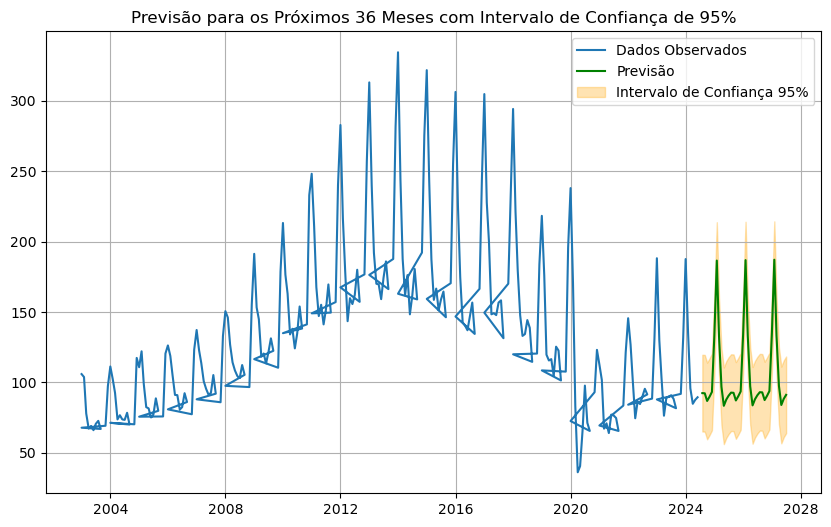
\includegraphics[scale = 0.7]{images/3.vii_ab.png}
\caption{Gráfico com intervalo de confiança}
\end{figure}

Além do gráfico, geramos a seguinte tabela contendo os resultados das predições.

\begin{figure}[H]
\centering
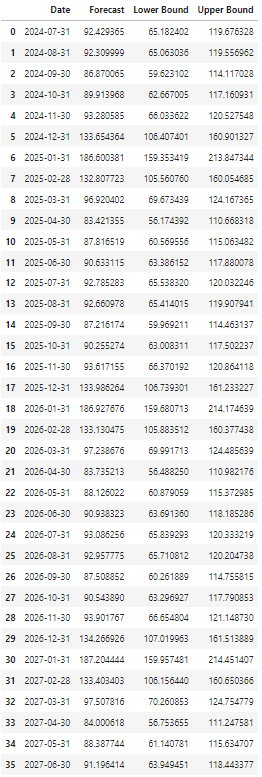
\includegraphics[scale = 1.5]{images/3.vii_table.png}
\caption{Tabela com previsões para 36 meses}
\label{filtro1}
\end{figure}


\textbf{Tendência Geral:}\\
No gráfico, vemos que a série original apresenta uma tendência decrescente a partir de 2016, com variações sazonais significativas ao longo dos anos. A previsão para os próximos 36 meses sugere uma leve recuperação da tendência, mas a maior parte das previsões ainda mostra valores relativamente baixos, mantendo uma oscilação sazonal.\\

\textbf{Comportamento Sazonal:}\\
A sazonalidade é evidente tanto na série original quanto nas previsões. Observa-se que os picos e vales sazonais são previstos para continuar de forma semelhante ao comportamento passado, com alguns períodos de alta nos primeiros meses do ano e quedas subsequentes.\\

\textbf{Intervalo de Confiança:}\\
O intervalo de confiança de 95\% mostrado em torno da linha de previsão (em amarelo) sugere uma incerteza considerável nos valores futuros. Quanto mais distante no tempo (mais próximo de 2027), maior a incerteza, refletida pelo alargamento do intervalo de confiança. Isso é comum em previsões de séries temporais, especialmente em séries com forte sazonalidade e variações abruptas.\\


\textbf{Previsão para os Próximos Meses:}\\
A tabela apresenta as previsões de vendas para cada mês, com um intervalo de confiança que indica o range dentro do qual o valor real de vendas pode cair com 95\% de probabilidade.
Por exemplo, a previsão para julho de 2024 (primeira linha) é de 92.43, com um intervalo de confiança que vai de 65.18 a 119.68. Isso significa que, com 95\% de certeza, as vendas em julho de 2024 devem estar entre esses valores.\\

\textbf{Variabilidade ao Longo do Tempo:}\\
Observa-se que os valores previstos seguem um padrão sazonal, com os meses de dezembro e janeiro tendo previsões significativamente mais altas (como 186.60 para janeiro de 2025). Isso reflete picos de vendas provavelmente relacionados a fatores sazonais, como festas de fim de ano.
Os valores de previsão e seus respectivos intervalos de confiança aumentam e diminuem em sincronia com os padrões sazonais passados, confirmando a consistência do modelo em capturar essa sazonalidade.\\


\textbf{Ponderando os Valores:}\\
O fato de os intervalos de confiança não serem simétricos (por exemplo, o intervalo de confiança para 2027-01-31 é de 159.96 a 214.45) indica que o modelo está capturando a assimetria na variação sazonal das vendas.\\
O menor valor de previsão (84.00 em 2027-04-30) sugere um período sazonalmente mais fraco para as vendas, enquanto os valores mais altos, como 187.20 em 2027-01-31, sugerem períodos sazonais de alta demanda.\\

Portanto, o modelo parece estar capturando bem a sazonalidade e a tendência decrescente da série. No entanto, a incerteza aumenta com o tempo, o que é normal em previsões de longo prazo.\\


\newpage
% REFERENCIAS %%%%%%%%%%%%%%%%%%%%%%%%%%%%%%%%%%%%%%%%%%%%%%%%%%%%%%%%%%%%%%



\end{document}